\section{Results}
\section{Results}

The simulation was conducted in GPGPU-Sim for NVIDIA Fermi GPU architecture \cite{bakhodayuan09}. GPGPU-Sim was configured to simulated the performance of GTX580, with all 16 streaming multiprocessors enabled (each CUDA streaming multiprocessor is represented as a single SIMT Core in GPGPU-Sim). Each streaming multiprocressor contains 48 warps, with 32 threads per warp (See Figure \ref{GTX580}). All sixteen SIMT cores share unified L2 cache.

\begin{figure}[ht!]
\centering
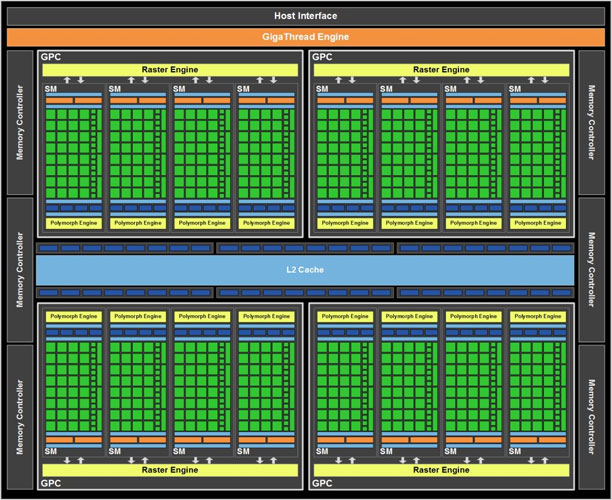
\includegraphics[width=90mm]{GTX580.jpg}
\caption{Block Diagram of Default GTX580. There are 16 SIMT Cores, all sharing a common L2 cache. Each SIMT Core contains a separate L1 cache.}
\label{GTX580}
\end{figure}

In the original Fermi architecture, each streaming multiprocessor has its own distinct L1 cache. Each L1 instruction cache is a 4-way set associative, with 4 sets of 128 bytes blocks. To assess the  performance of different L1 instruction cache architecture, only the L1 instruction cache was modified, while all other variables remained constant. Other aspects of the architecture such as the bandwidth of shared L2 cache could serve as a performance bottleneck for different cache designs. However, these variables are assumed to have little impact on the hit and stall rate of the instruction cache, which are the primary metrics of interest.

\jbs{More Content on Expected Results Coming...}

\begin{figure}[ht!]
\centering
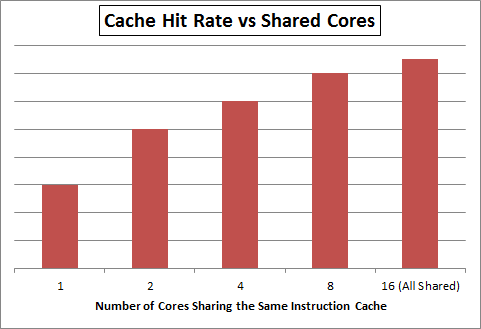
\includegraphics[width=90mm]{HitRateImprov.png}
\caption{Projected Improvement in Hit Rate. Total size of the instruction cache remains constant. Size of individual instruction cache is scaled proportionally to the number of cores that share the cache.}
\label{HitImprov}
\end{figure}

\begin{figure}[ht!]
\centering
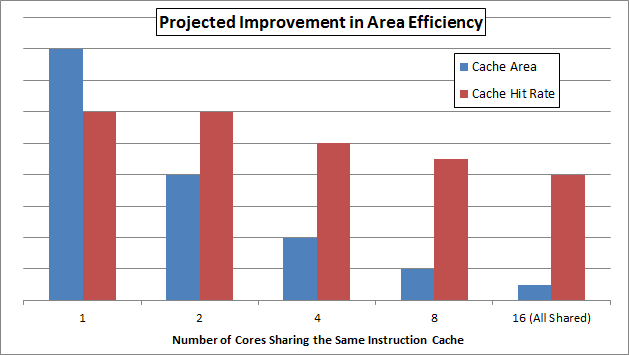
\includegraphics[width=90mm]{AreaEff.png}
\caption{Projected Improvement in Area Efficiency. Size of individual instruction cache remains constant, while the number of cores sharing the L1 cache is increased. The instruction redundancy between the cores should allow cache hit rate to remain high as cache area is reduced. }
\label{AreaEff}
\end{figure}

\subsection{Benchmarks}
Describe benchmarks used \jbs{Akhil in charge.}

\subsection{Preliminary Results}
\jbs{Fabiha in charge}

